\documentclass[dvips,ruledheader]{abnt}
\usepackage[brazil]{babel}
\usepackage[latin1]{inputenc}
\usepackage[dvips]{graphicx}
\usepackage{abnt-alf}
\usepackage{latexsym}
\usepackage{psfrag}
\usepackage[center]{caption2}
\usepackage{amsfonts}
\usepackage{float}
\usepackage{color}


\floatstyle{ruled}
\newfloat{listagem}{htbp}{listagem}
\floatname{listagem}{Listagem}


\begin{document}

\DeclareGraphicsRule{.eps.gz}{eps}{.eps.bb}{`gunzip -c #1}

\titulo{Reconhecimento e Busca Adaptativos de Padr�es Musicais}

\autor{Pedro Rodrigues Nacione Pedruzzi\\Ricardo A. Redder Jr.}

\orientador{Prof. Doutor Jo�o Jos� Neto}

\comentario{Disserta��o apresentada � Comiss�o de Gradua��o em Engenharia da Computa��o
 da Escola Polit�cnica da Universidade de S�o Paulo para a obten��o da gradua��o no curso
 de Engenharia da Computa��o.}

\instituicao{Gradua��o em Engenharia de Computa��o \par 
	Departamento de Computa��o e Sistemas Digitais \par 
	Escola Polit�cnica da Universidade de S�o Paulo}

\local{S�o Paulo -- SP}

\data{Dezembro / 2008}

\capa

\folhaderosto


\pretextualchapter{}

\vspace{17.5cm}
\begin{flushright}

\textit{``A m�sica escondida n�o tem valor.''
	\\\bfseries Aulo G�lio}

\end{flushright}




\begin{resumo}

Este trabalho prop�e uma nova forma de compara��o de conte�dos de �udio formados por melodias, baseando-se em t�cnicas adaptativas, em espec�fico, utilizando-se um aut�mato adaptativo. Para avalia��o deste m�todo um prot�tipo de um sistema de busca de �udio baseado em conte�do � proposto, abrangendo a captura de �udio, a compara��o, a busca e a sele��o dos conte�dos mais similares.

A arquitetura deste prot�tipo � apresentada, assim como o detalhamento de cada componente, mostrando o funcionamento e apresentando os resultados de cada fase do processo. Um foco maior � dado ao componente de compara��o adaptativo, por�m, o trabalho n�o deixa de apresentar um prot�tipo que valide os conceitos apresentados, al�m de permitir a avalia��o do desempenho do processo como um todo.

\end{resumo}


\begin{abstract}

This work proposes a different method of comparing audio content composed by melodies, based on adaptative techniques, specifically, using an adptative automaton. For the evaluation of this method, a prototype of an audio content-based search engine is proposed, comprehending the audio capture, the comparison, the search and the selection of the most similar content.

The architecture of this prototype is presented, as well as the details of each component, showing the operation and presenting the results of each phase of the process. A major focus is given to the adaptative comparison component, nevertheless, the work still presents a prototype which may validates the proposed concepts, besides that, it enables the evaluation of the process performance as whole.

\end{abstract}


\setcounter{tocdepth}{3}
\tableofcontents

\listoffigures
\listoftables
% \listof{listagem}{Lista de Listagens}

\chapter*{Introdu��o}

Sistemas de busca de texto j� se tornaram parte do cotidiano das pessoas ao redor do mundo, evolu�ram desde prot�tipos desenvolvidos em laborat�rios de universidades at� se tornarem enormes e complexos sistemas comerciais. Apesar disso, estes sistemas ainda se ap�iam fortemente sobre algoritmos de compara��o de doscumentos, que procuram avaliar o grau de similaridade entre dois documentos dados.

Com a populariza��o cada vez maior de conte�dos de multim�dia, surge o interesse por extender a id�ia de sistemas de busca para esta �rea de informa��o. Dentre a vastid�o de pesquisas que abordam o tema, um tema de grande interesse � a busca de conte�dos de �udio baseados em conte�do. Este trabalho aborda tal tema, se focando em especial em um m�todo de compara��o de conte�dos de �udio, baseado em t�cnicas adaptativas. O m�todo de compara��o desenvolvido termina por servir de base para a implanta��o de um prot�tipo de um sistema de busca, envolvendo captura de �udio, identifica��o de notas, compara��o e busca. 

Em suma, o prot�tipo desenvolvido se prop�em a identificar uma m�sica reproduzida por um usu�rio atrav�s de um assobio. Ap�s o detalhamento do prot�tipo, testes com o sistema s�o apresentados, assim como seus resultados, a fim de permitir uma avalia��o inicial do m�todo desenvolvido.

Por fim, uma an�lise do trabalho � desenvolvida, apontando seus pontos de melhoria, contribui��es, extens�es e trabalhos futuros. Assim, espera-se poder contribuir com esta crescente �rea de pesquisa que � a recupera��o de informa��o em conte�dos mult�midia, a partir da utiliza��o de uma t�cnica adaptativa, e ao mesmo tempo, pretende-se poder contribuir tamb�m com o estudo da adaptatividade, com esta interessante aplica��o do conceito.

% Define keywords, ou atalhos para serem usados ao longo do texto

\newcommand{\query}{{\em query}}




\chapter{Motiva��o}

Os sistemas de busca atuais evolu�ram rapidamente desde suas primeiras vers�es, e hoje se tornaram parte fundamental do cotidiano de grande parte da popula��o. Para muitos profissionais � dif�cil imaginar um dia de trabalho em que n�o se utilize algum mecanismo de busca. Pode-se citar como exemplo destes sistemas: Google.com \texttrademark, Yahoo.com \texttrademark \ ou Live Search \texttrademark.

Por�m tais sistemas de busca em geral baseiam-se sobre os mesmos princ�pios e m�todos de busca, em sua maioria aplicados ao dom�nio textual. Mesmo alguns sistemas que, por exemplo, efetuam buscas por imagens ou v�deos continuam em sua ess�ncia baseando-se nos mesmos princ�pios, j� que se ap�iam na categoriza��o textual do conte�do.

A populariza��o destes sistemas de busca mostrou as possibilidades de expans�o e a import�ncia que estes podem adquirir no cotidiano pessoal e profissional das pessoas. Por�m suas limita��es de contexto (restri��o a textos apenas) imediatamente levantam a necessidade de novas t�cnicas com o fim de ampliar os dom�nios de aplica��o destes sistemas.

Um dos dom�nios de extrema import�ncia com rela��o a tal tema � o dom�nio de �udio, devido a fatores como sua popularidade no meio virtual, quantidade de conte�do dispon�vel, facilidade de produ��o de conte�do, etc. M�sicas em formatos digitais, tais como MP3, MIDI, WAV, etc, podem ser facilmente encontradas na internet e j� se tornaram parte do cotidiano de grande parte da popula��o. Al�m disso, a capacidade de reproduzir tais formatos torna-se cada vez mais um padr�o nos aparelhos eletr�nicos de �udio. Paralelamente aos conte�dos de �udio digitais, podem-se citar ainda conte�dos de �udio-visual, que recentemente adquiriram grande popularidade e, analogamente aos conte�dos de �udio, est�o cada vez mais se tornando parte importante do ambiente virtual.

Uma situa��o t�pica e extremamente frequente, � aquela na qual um indiv�duo � capaz de reproduzir apenas um trecho da melodia de uma m�sica que deseja encontrar. Tal reprodu��o est� inerentemente sujeita a varia��es de diversas naturezas com rela��o � melodia original. O indiv�duo pode reproduzir a melodia com diverg�ncias na altura (frequ�ncia fundamental de vibra��o) ou dura��o das notas musicais, ou pode ainda cometer erros com rela��o a pr�pria melodia, como por exemplo, esquecendo uma nota ou inserindo uma nota inexistente. Este caso pode manifestar-se a partir de diversas situa��es do cotidiano, como ao tentar encontrar uma m�sica ouvida em um filme, um programa de televis�o ou r�dio, etc.

Este tipo de problema � extremamente dif�cil para um indiv�duo comum devido � falta de ferramentas que possam auxiliar tal busca, j� que a grande quantidade de m�sicas existentes torna invi�vel uma varredura completa dos reposit�rios existentes, ou seja, ouvir todas as m�sicas, uma a uma. Al�m disso, as formas mais comuns de organiza��o de reposit�rios musicais recaem sobre estilos musicais e nomes, o que n�o � o suficiente para endere�ar, ou ajudar no problema apresentado, j� que, em geral, tais informa��es n�o s�o suficientes para encontrar uma m�sica a partir de um trecho de uma de suas melodias.

Atualmente, a forma mais comum de tentar encontrar uma solu��o para tal problema � utilizando-se a ajuda de um especialista (um vendendor de discos, por exemplo), que em alguns casos, � capaz de identificar o trecho reproduzido. O problema imediato com tal abordagem � o fato da mesma n�o ser escal�vel e de dif�cil utiliza��o, al�m de enfrentar limita��es impostas pela pr�pria natureza do especialista, como dificuldade de lidar com grandes quantidades de m�sicas, diversidades de estilo, etc.

Assim, apesar da grande relev�ncia de conte�dos multim�dia e dos incont�veis esfor�os de pesquisa na �rea, diversas quest�es ainda permacenem em aberto. Poucos s�o os mecanismos de busca j� em est�gio maduro capazes de lidar com tais conte�dos. Dentre tais quest�es em aberto, uma de extrema relev�ncia � a similaridade entre conte�dos de �udio. Onde, apesar das diversas t�cnicas j� utilizadas, dificuldades no estabelecimento do significado da similaridade entre dois conte�dos ainda permanece. Al�m disso, o estabelecimento de um algoritmo de similaridade eficaz serve como um dos pilares para um bom sistema de busca, j� que diversos m�todos de busca se ap�iam em tal medida.

Sistemas capazes de identificar m�sicas automaticamente a partir de uma amostra reduzida tamb�m teriam uma grande aplica��o na detec��o de pl�gios e usos n�o autorizados. A fiscaliza��o de uso n�o autorizado de m�sicas ou trilhas musicais � particularmente dif�cil, pois ap�s a sua vincula��o dificilmente t�m-se um rastro de sua utiliza��o, e a identifica��o de um pl�gio � bastante subjetiva. Sistemas de identifica��o autom�tica seriam capazes de fornecer fortes ind�cios de ambos os casos. Basta imaginar que um sistema como esse poderia monitorar uma transmiss�o de r�dio ou TV, verificando se h� similaridade com um dado conte�do. Uma alta similaridade poderia dar ind�cio de um uso n�o autorizado ou um pl�gio deste conte�do.

Estes fatos demonstram a demanda por avan�os que possam auxiliar tal tipo de busca, ou seja, a necessidade por ferramentas ou algoritmos que permitam o avan�o da �rea de recupera��o de informa��o multim�dia. E � justamente neste ponto que este trabalho se encaixa, na tentativa de propor mais uma ferramenta para compara��o de conte�dos de �udio, em especial, conte�dos compostos por melodias, ou sequ�ncia de notas.

\chapter{Objetivo}

Atrav�s deste projeto deseja-se abordar uma quest�o extremamente ampla, que � a busca sobre conte�dos de �udio, por�m, por ser um tema vasto, uma redu��o de escopo para os fins deste projeto se faz necess�ria. Assim decidiu-se por focar-se nos pontos de maior relev�ncia para o problema.

Um dos pontos que estabelece a maior barreira para a constru��o de um sistema como o vislumbrado � a dificuldade de compara��o entre dois conte�dos de �udio. Esta compara��o n�o � bem definida, assim n�o h� uma forma consistente de se estabelecer o conceito de dist�ncia entre dois conte�dos de �udio, conceito que por sua vez � fundamental para a utiliza��o dos modelos de busca e indexa��o existentes.

Assim, pretende-se com este trabalho promover um avan�o sobre tal quest�o de compara��o de conte�dos de �udio, e para tanto, ser�o adotadas t�cnicas pouco exploradas em tal dom�nio. O projeto se apoiar� sobre dois pilares importantes: a utiliza��o de conceitos do dom�nio musical e o uso de t�cnicas adaptativas, ambos aplicados � compara��o de conte�dos de �udio.

Diversas t�cnicas t�m sido utilizadas para an�lise e compara��o de sinais de �udio, por�m, em sua maioria, tais m�todos recaem sobre princ�pios de processamento de sinais, por serem gen�ricos e possu�rem grande aplicabilidade, tendendo a ignorar conceitos espec�ficos do dom�nio musical, ou seja, conceitos de notas, tempos, etc. Entretanto, tais princ�pios podem ser de grande relev�ncia quando se deseja efetuar uma busca por m�sicas. Assim, com este trabalho, aspira-se a utiliza��o de tais conceitos dentro do contexto de compara��o de conte�dos de �udio, com o fim de obter melhores resultados.

Paralelamente a isto, deseja-se utilizar t�cnicas adaptativas no esfor�o de se obter um m�todo de compara��o entre trechos de �udio. A id�ia � criar um aut�mato adaptativo baseado em um trecho de �udio, e assim, um segundo trecho de �udio que submetido a este aut�mato geraria uma sa�da que conteria uma indica��o da dist�ncia entre os dois trechos. Esta dist�ncia, reconhecida pelo aut�mato, entre dois trechos de �udio poderia servir como base de entrada para outros algoritmos tradicionais de ranking.
Da jun��o destes conceitos e ferramentas espera-se criar um sistema capaz de receber um trecho de �udio de um usu�rio e identificar dentro de um reposit�rio limitado qual m�sica se corresponde ao trecho reproduzido pelo usu�rio.
\chapter{Hist�rico}

Nesta se��o ser�o apresentados os hist�ricos dos principais temas relacionados ao projeto desenvolvido. Mostrando sucintamente a hist�ria que se desenrolou paralelamente dos sistemas de busca e dos avan�os dos m�todos de manipula��o de conte�dos de �udio atrav�s dos computadores.

\section{Hist�rico dos sistemas de busca}

M�todos de busca baseados em texto j� s�o antigos e utilizados h� um longo tempo, entre os m�todos mais simples pode-se citar o uso �ndices remissivos. Apesar de simples, este m�todo � extremamente �til e eficiente quando se deseja buscar por uma palavra dentro de um conjunto de documentos. Al�m deste m�todo simples, existem ainda outras formas de se indexar um documento e efetuar uma busca sobre o mesmo. Por�m a aplica��o manual destes m�todos sempre apresentou dificuldades, pelas dificuldades de indexa��o de palavras, lentid�o de busca, etc.

Como advento dos computadores, tais m�todo passaram a ser implantados por computadores, o que obviamente aumentou sua capacidade, e facilidade de uso. Assim nasceram os primeiros sistemas de busca, juntamente com os computadores. Por�m estes m�todos eram em sua ess�ncia muito simplistas, considerando em geral apenas buscas por trechos exatos.

A id�ia dos sistemas de busca da forma como conhecemos hoje surgiu algum tempo depois, j� por volta da d�cada de 60, e foi se aprimorando ao longo dos anos. Conceitos como modelo de espa�o vetorial, frequ�ncia inversa no documento (IDF), frequ�ncia do termo (TF), discrimina��o de termos, relev�ncia e feedback come�aram a ser galgados nesta �poca. Tais t�cnicas evolu�ram muito ao longo dos anos, provendo ferramentas extremamente importantes para efetuar indexa��o e buscas sobre conjuntos extensos de documentos.

Conforme o tamanho do espa�o de busca cresce, maior import�ncia tais t�cnicas assumem, assim, com o advento da internet, estes m�todos adquiriram um papel especial no mundo da computa��o. Isso porque a internet abriu a possibilidade de se criar espa�os de buscas muito maiores do que at� ent�o constru�dos, j� que a superf�cie de busca poderia ser virtualmente todo documento dispon�vel na rede. 
Por volta da d�cada de 90 come�am ent�o a surgir os sistemas web de indexa��o e busca, o primeiro sistema deste tipo foi o Archie, porem efetuava buscas apenas sobre nomes de arquivos, e n�o sobre seus conte�dos. Pouco tempo depois surgiram os primeiros crawlers, componente dos sistemas de busca que se tornou indispens�vel aos sistemas atuais.

Desde seu in�cio at� o presente a ci�ncia de Recupera��o de Informa��o (Information Retrieval) evolui muito, e diversos m�todos de busca, al�m de varia��es, foram criados ao longo destes anos, e hoje se podem citar dois modelos que assumiram import�ncia fundamental nesta ci�ncia o modelo espa�o vetorial, e o modelo probabil�stico.

Tais modelos e t�cnicas d�o o tom do estudo desta ci�ncia no mundo acad�mico, por�m apenas tais conceitos n�o s�o o suficiente para se construir um sistema de busca similar aos que encontramos atualmente. Al�m destes princ�pios, considera��es diversas relacionadas a desempenho, propriedade intelectual, conte�do impr�prio, conte�do falso, tentativas de manipula��o de resultados, etc. devem ser levadas em conta.
Hoje, uma das tend�ncias mais fortes de desenvolvimento desta �rea � a especializa��o dos sistemas de buscas, levando em conta, por exemplo, aspectos sem�nticos do tema que constitui o espa�o de busca. Relacionado a isso, h� tamb�m um grande interesse em expandir as fronteiras da ci�ncia de recupera��o de informa��o para outros tipos de conte�do, como conte�dos de �udio e v�deo. Recentemente, a TREC - Text REtrieval conference, uma das maiores confer�ncias sobre recupera��o de texto, incorporou o tema de busca sobre �udio como uma sub-tarefa.

\section{Hist�rico de t�cnicas de estima��o de frequ�ncia}
O problema de estimar a frequ�ncia de trecho de �udio � um problema estudado h� um longo tempo, diversas t�cnicas e m�todos j� foram desenvolvidos sobre o tema, por�m at� o presente momento estas t�cnicas ainda apresentam fortes defici�ncias e n�o s�o capazes de atingir o n�vel desejado de qualidade. Frente a um sinal �nico claro, diversas t�cnicas apresentam um bom desempenho, por�m quando testadas com sinais ruidosos, ou contendo mais de uma linha mel�dica estas t�cnicas tendem a falhar.
Diferentes conceitos podem ser aplicados na tentativa de estimar a frequ�ncia de um trecho de �udio, entre as principais t�cnicas tem-se: m�todos que se baseiam no dom�nio do tempo, m�todos que utilizam o dom�nio da frequ�ncia e m�todos estat�sticos.

M�todos baseados na an�lise do dom�nio do tempo se valem do fato que os sinais s�o peri�dicos, o que faz alguns eventos tamb�m serem peri�dicos, e, portanto, podem ser contados.

\paragraph{Taxa de cruzamento do eixo (ZCR - Zero-crossing rate).} A id�ia deste m�todo consiste em contar o n�mero de vezes que o sinal de �udio cruza o eixo dos tempos, imaginando-se que a principal componente de frequ�ncia respons�vel por este cruzamento ser� a frequ�ncia fundamental. A Figura \ref{fig:zcr} exemplifica o fato, onde uma componente de frequ�ncia mais alta n�o exerce grande influ�ncia sobre o n�mero de cruzamentos do sinal com o eixo dos tempos.

\begin{figure}[htb]
	\center{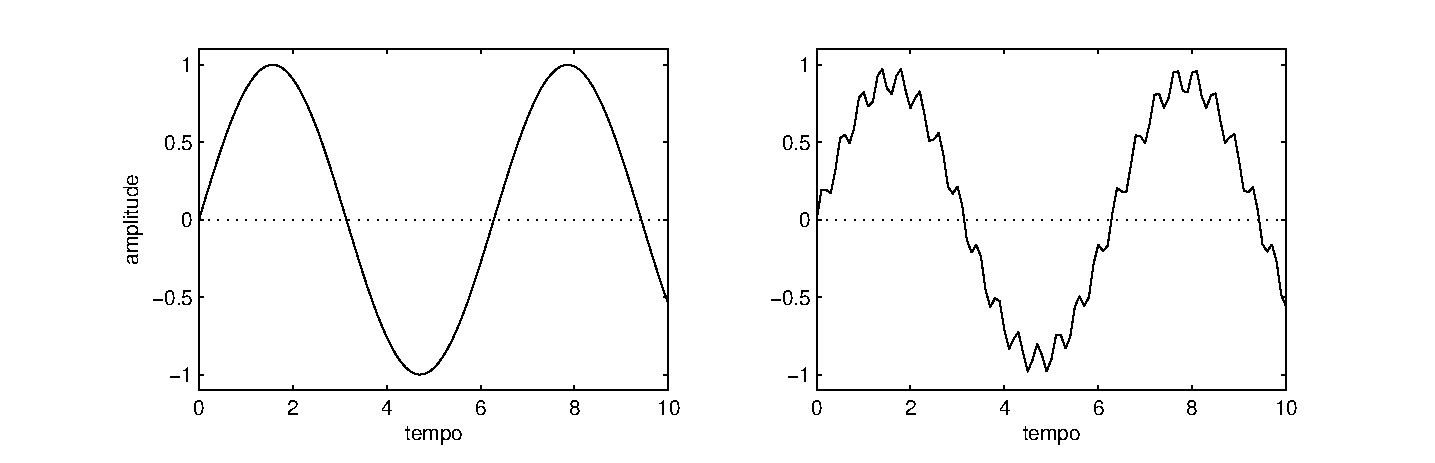
\includegraphics[width=\textwidth]{figuras/zcr.eps}}
	\caption{\label{fig:zcr} Influ�ncia da frequ�ncia fundamental na taxa de cruzamento do eixo}
\end{figure}

\paragraph{Taxa de picos.} Este m�todo consiste em contar o n�mero de picos por segundo em um sinal, sabendo que atrav�s do n�mero de picos � poss�vel inferir a frequ�ncia do sinal, tem-se ent�o a estimativa do frequ�ncia. Analogamente ao ZCR, a frequ�ncia fundamental ser� a componente de frequ�ncia que mais contribuir� para a ocorr�ncia de picos no sinal, assim � poss�vel dizer que a estimativa obtida corresponde � estimativa da frequ�ncia fundamental.

\paragraph{Taxa de eventos de inclina��o.} Devido ao fato do sinal ser peri�dico a inclina��o do sinal tamb�m ir� variar periodicamente, assim observar picos e zeros da inclina��o do sinal pode ser mais informativo do que observar picos e zeros do sinal original.

\paragraph{Correla��o.} Existem ainda m�todos que se baseiam na correla��o entre duas amostras de �udio, definindo assim a similaridade entre os dois sinais. Formas de onde similares apresentariam uma correla��o alta, enquanto formas de onda muito diferentes teriam uma baixa correla��o.

Al�m de m�todos baseados no dom�nio do tempo, existem tamb�m diversas t�cnicas baseadas no dom�nio da frequ�ncia. Estas, por sua vez, recaem sobre o fato de que o sinal pode ser modelado como uma soma de s�ries harm�nicas, guardando um alto grau de informa��o sobre a frequ�ncia fundamental.

\paragraph{Propor��o de componentes de frequ�ncia}  Em 1979, Martin Piszczalski trabalhava em um sistema capaz de transcrever m�sicas automaticamente, assim, necessariamente um dos componentes deste sistema era o componente de extra��o de notas. O procedimento adotado se valia do c�lculo do espectro do sinal, da detec��o de picos deste espectro, e de uma an�lise probabil�stica destes picos.

\paragraph{M�todos baseados em filtros} Estes m�todos utilizam a id�ia de aplicar diferentes filtros ao sinal, e analisar sua sa�da. Por exemplo, caso um sinal possua uma sa�da alta ap�s a aplica��o de um filtro passa-faixa, pode-se afirmar que este sinal possui entre suas componentes a frequ�ncia do filtro. Em 1977 James A. Moorer, propos um algoritmo denominado Filtro Comb �timo, baseado nestes conceitos. Uma tentativa mais recente foi proposta por John E. Lane, denominado Filtro IIR Ajust�vel. Existem ainda diversas t�cnicas que se ap�iam sobre a an�lise cepstrum, que corresponde ao resultado da tranformada de Fourier do log do espectro de magnitude so sinal de entrada.

Diversos m�todos estat�sticos sobre o dom�nio da frequ�ncia tamb�m foram desenvolvidos, dentre estes deve-se destacar duas abordagens importantes: redes neurais e estimadores de M�xima Verossimilhan�a.
\chapter{Resenha bibliogr�fica}

Na presente se��o ser�o apresentados as diversas t�cnicas nas quais este trabalho se fundamenta. Al�m de uma vis�o geral dos aspectos fundamentais de cada assunto, s�o dadas refer�ncias para material detalhado para o completo entendimento destes.

\section{Processamento de sinais}
\subsection{Transformada r�pida de Fourier}

\section{M�todo dos m�nimos quadrados}

O m�todo dos m�nimos quadrados � uma t�cnica matem�tica de otimiza��o que surgiu no in�cio do s�culo XIX, por�m amplamente utilizada at� os dias atuais. Este m�todo permite encontrar os par�metros para uma fun��o modelo $f$ de forma a melhor aproximar uma rela��o entre grandezas. Esta rela��o � usualmente dada por um conjunto de pares ordenados $(x_i,y_i)$. Neste caso, se imaginarmos que $f(x_i) \approx y_i$, deseja-se ajustar seus par�metros de modo a minimizar a soma dos quadrados dos erros: $$S = \sum_{i=1}^n (y_i - f(x_i))^2$$

A teoria mostra que para o caso em que a fun��o modelo $f$ � linear com rela��o aos seus par�metros, a solu��o para o problema � �nica e ocorre quando as derivadas parciais do erro quadr�tico com rela��o a cada par�metro � zero. Estas equa��es resultam em um sistema linear poss�vel e determinado, de forma que a solu��o pode ser facilmente obtida utilizando os m�todos num�ricos de resolu��o de sistemas lineares.

Para um aprofundamento sobre o m�todo dos m�nimos quadrados ou sobre m�todos de resolu��o de sistemas lineares, consulte a efer�ncia ~\ref{calculoNumerico}.

\section{Tecnologia adaptativa}

~\ref{roteiroLTA}
~\ref{Neto94}
Adaptatividade � um conceito 
Laborat�rio de Linguagens e T�cnicas Adaptativas

Uso de dispositivos adaptativos. Formalismos computacionais com capacidade de auto-reconfigura��o din�mica (em execu��o).

linguagens formais e aut�matos, complexidade computacional, modelos de computa��o, paradigmas de programa��o sintaxe e sem�ntica formal, m�quinas virtuais, ambientes de execu��o.


A maior vantagem dos dispositivos adaptativos � a sua facilidade de uso, sua relativa simplicidade e o fato de ser muito rara a necessidade de existir uma descri��o completamente especificada do comportamento do dispositivo para que ele possa ser utilizado. Em lugar disso, sua opera��o pode ser descrita de forma incremental, e seu comportamento, programado para se alterar dinamicamente em resposta aos est�mulos de entrada recebidos. Adicionalmente, como o conjunto de regras que definem o seu comportamento tamb�m se altera ao longo da sua opera��o, pode-se dizer que o pr�prio dispositivo adaptativo implementa de alguma forma a representa��o do conhecimento adquirido atrav�s de sua seq��ncia recebida de est�mulos de entrada.

\chapter{Conceitos}

Este cap�tulo apresentar� a forma como os conceitos presentes no trabalho se interligaram, mostrando o sistema proposto, suas principais caracter�sticas, componentes e funcionalidades.

\section{Sistema}


\subsection{Descri��o}

Prop�e-se o desenvolvimento de um prot�tipo de um sistema de buscas por m�sicas baseado em conte�do, este sistema recebe uma entrada do usu�rio que corresponde � sua \query, ou seja, algum trecho da m�sica buscada que o usu�rio reproduza atrav�s de um assobio. O sistema recebe a \query \ e em seguida compara com as m�sicas presentes em seu reposit�rio, calculando a similaridade entre cada m�sica e a \query, a partir das compara��es efetuadas, o sistema � capaz de apresentar quais as entradas mais prov�veis de corresponderem � m�sica procurada.

Em linhas gerais, a id�ia de uso do sistema pode ser vista na Figura ~\ref{fig:usecase}.

\begin{figure}[htb]
	\center{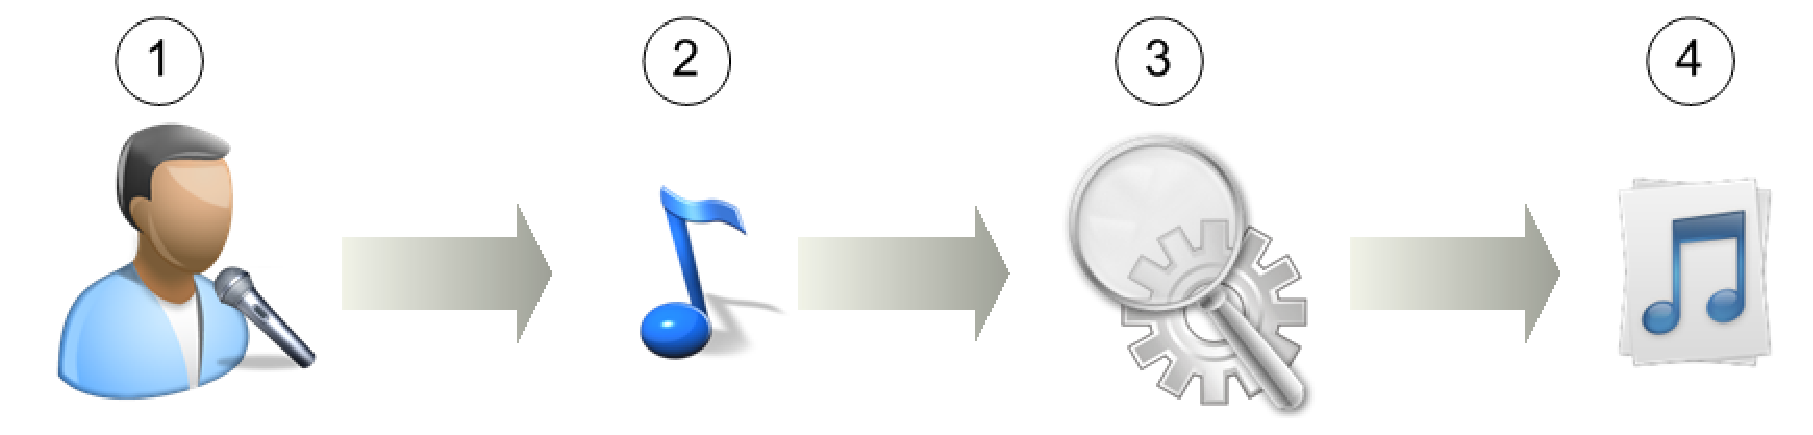
\includegraphics[width=0.7\textwidth]{figuras/usecase.eps}}
	\caption{\label{fig:usecase} Caso de uso t�pico do sistema}
\end{figure}

\begin{enumerate}
\item Usu�rio do sistema
\item Trecho de m�sica (ou conte�do) gerado pelo usu�rio
\item Sistema de busca
\item Conjunto de m�sicas mais pr�ximas do trecho gerado pelo usu�rio
\end{enumerate}



\subsubsection{Espa�o de busca}

O espa�o de busca � constitu�do por m�sicas em formato MIDI, devidamente preparadas para o ambiente de execu��o de buscas. Pelo fato dos arquivos MIDI, na maioria dos casos, possuirem diversas trilhas, devem portanto passar por um processo de prepara��o, onde apenas a trilha mais relevante da m�sica � extra�da e ent�o adicionada ao reposit�rio. Devido ao foco dado ao sistema este processo se desenvolve manualmente, atrav�s de uma an�lise humana de cada trilha, escolhendo a mais relevante.


\subsubsection{Entrada de dados}

o usu�rio deve fornecer como entrada ao sistema um assobio de um trecho de uma m�sica que deseja buscar, originando a \query \ que ser� processada. As informa��es fornecidas pelo usu�rio, em geral, s�o muito limitadas e com grandes varia��es com rela��o ao conte�do original, al�m disso tipicamente o trecho � curto e erros s�o frequentes. Para fins de processamento da \query \ a origem da mesma � irrelevante, assim, outras formas de entrada que gerassem notas musicais, como um piano por exemplo, seriam pass�veis de utiliza��o.


\subsection{Arquitetura do Sistema}

A arquitetura proposta para o prot�tipo � dividida em componentes, conforme pode ser visto na Figura ~\ref{fig:arquitetura}, cada componente procura implantar uma fun��o bem determinada, de modo que seja facilmente troc�vel, isso d� abertura para uma evolu��o cont�nua do prot�tipo.

\paragraph*{Vis�o geral} O usu�rio dever� fornecer a entrado ao sistema, que por sua vez, digitalizar� e converter� o sinal para um modelo musical que representar� o trecho fornecido, ou seja, a \query. Em seguida, esta ser� apresentada ao componente de busca do sistema, que analisar� a mesma comparando-a com as m�sicas existentes no reposit�rio. Um dos pilares da compara��o � a adaptatividade, que ajusta o comparador principal. Ao fim da compara��o com as entradas do reposit�rio, � poss�vel estabelecer o conjunto de m�sicas mais prov�veis de atender � \query \ do usu�rio.

\begin{figure}[htb]
	\center{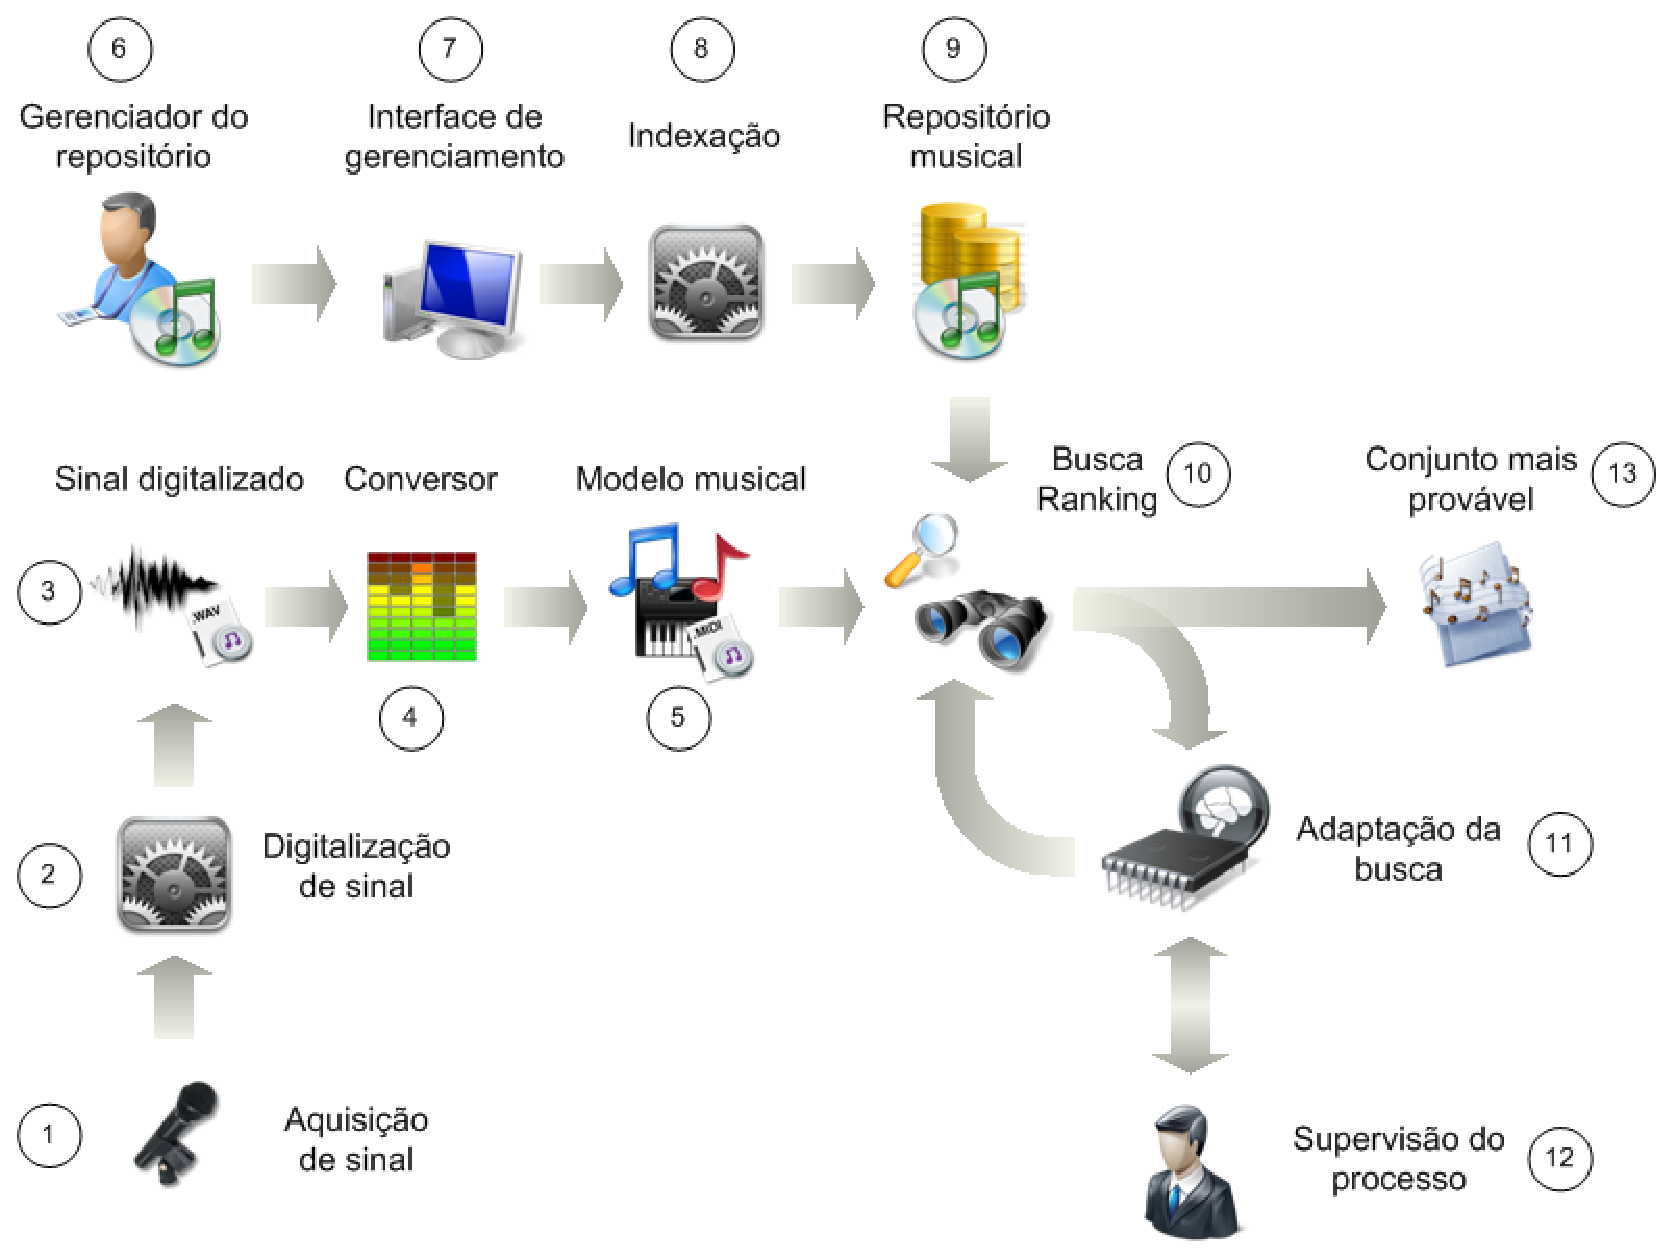
\includegraphics[width=0.85\textwidth]{figuras/arquitetura.eps}}
	\caption{\label{fig:arquitetura} Arquitetura do sistema}
\end{figure}

Componentes da arquitetura:

\begin{enumerate}

\item Equipamento de captura de �udio (ex.: microfone).

\item Digitalizador do sinal. Converte o sinal gerado pelo usu�rio em um sinal digitalizado,.

\item Sinal digitalizado. Armazena o sinal digitalizado gerado pelo usu�rio, em um formato WAV. At� este ponto as perdas de informa��o devido �s convers�es e transforma��es s�o irrelevantes.

\item Conversor. Tem por fun��o converter o sinal digitalizado, para um modelo musical. Este conversor dever� extrair informa��es musicais relevantes, como notas, tempos, etc.

\item Modelo musical. A sa�da do conversor ser� o modelo musical que descreve o sinal gerado pelo usu�rio. Este modelo musical deve armazenar informa��es no dom�nio musical, como notas e tempos.

\item Gerenciador do reposit�rio. Consiste de um operador que alimentar� o reposit�rio musical, definindo o espa�o de busca.

\item Interface de gerenciamento. Permite a adi��o ou remo��o de m�sicas no reposit�rio musical, age simplesmente como interface para a indexa��o.

\item Indexa��o. Este componente receber� a m�sica adicionada pela interface de gerenciamento e dever� process�-la e prepar�-la para ser armazenada ao reposit�rio musical. Essa prepara��o consiste da extra��o da cadeia que representa a m�sica e de sua trilha mais relevante.

\item Reposit�rio musical. Armazena os modelos musicais das m�sicas adicionadas atrav�s da interface de gerenciamento.

\item Busca e ranking. Procurar� dentro do reposit�rio musical os modelos mais prov�veis de terem gerado o sinal de entrada do usu�rio. Al�m disso, os modelos escolhidos como conjunto de resposta devem ser comparados de forma a exibir ao usu�rio uma lista por ordem de relev�ncia, ou seja, a lista deve possuir as entradas mais prov�veis de corresponderem � m�sica procurada no seu topo.

\item Adapta��o da busca. Alimenta e interfere na compara��o utilizada pela busca, mudando as regras utilizadas durante a busca e ranking. Este componente empregar� t�cnicas adaptativas.

\item Supervis�o do processo. Tem a fun��o de avaliar as respostas do sistema, avaliando o mesmo, a fim de guiar as altera��es.

\item Conjunto mais prov�vel. Resposta do sistema � pesquisa efetuada pelo usu�rio, com os resultados de melhor desempenho.

\end{enumerate}
\chapter{T�cnicas e procedimentos usados}
\label{chap:tecnicas}

Este cap�tulo descreve detalhes do sistema desenvolvido, apresentando sua especifica��o, detalhes de t�cnicas utilizadas, al�m de procedimentos envolvidos.

\section{Especifica��o do sistema}

Prop�e-se o desenvolvimento de um m�dulo de busca por m�sicas baseado em conte�do apoiado em t�cnicas adaptativas, e para teste e avalia��o da tecnologia empregada um prot�tipo de um sistema mais completo ser� constru�do.

\subsection{Descri��o}

A id�ia geral de um sistema de busca est� impl�cita na maioria das pessoas que se utilizam de servi�os como os de busca por documentos, nestes servi�os, em geral o usu�rio entra com um trecho do documento que ele procura, e o sistema de busca encontra documentos que mais se aproximem do trecho que o usu�rio proveu. Analogamente, em um sistema de busca por �udio baseado em conste�do, o usu�rio prov� um trecho do �udio que deseja encontrar, e o sistema encontra os �udios mais similares.

\subsection{Uso do sistema}

Prop�e-se o desenvolvimento de um prot�tipo de um sistema de buscas por m�sicas baseado em conte�do, que receba uma entrada do usu�rio que corresponde � sua \query, ou seja, algum trecho da m�sica buscada que o usu�rio reproduza atrav�s de um assobio, e em seguida compara com as m�sicas presentes em seu reposit�rio, calculando a similaridade entre cada m�sica e a \query, a partir das compara��es efetuadas, o sistema � capaz de apresentar quais as entradas mais prov�veis de corresponderem � m�sica procurada.

Em linhas gerais, a id�ia de uso do sistema pode ser vista na Figura ~\ref{fig:usecase}.

\begin{figure}[htb]
	\center{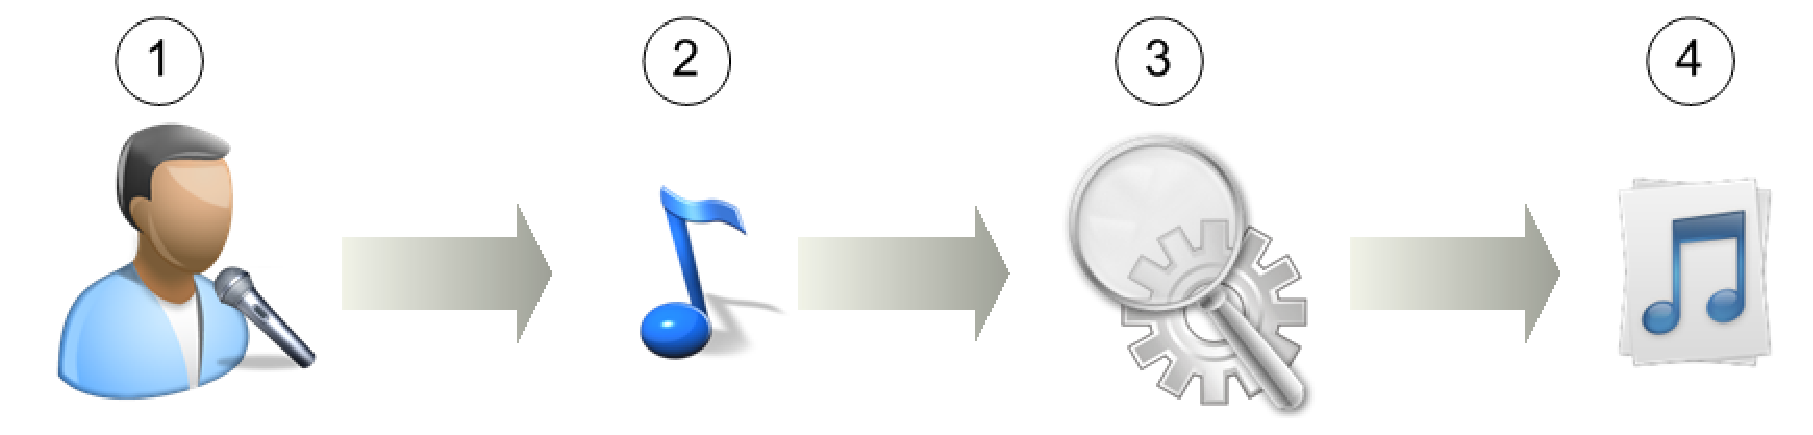
\includegraphics[width=0.7\textwidth]{figuras/usecase.eps}}
	\caption{\label{fig:usecase} Caso de uso t�pico do sistema}
\end{figure}

\begin{enumerate}
\item Usu�rio do sistema
\item Trecho de m�sica (ou conte�do) gerado pelo usu�rio
\item Sistema de busca
\item Conjunto de m�sicas mais pr�ximas do trecho gerado pelo usu�rio
\end{enumerate}

\subsection{Requisitos funcionais e Premissas}

Apesar da id�ia ser simples, sua complexidade � grande, assim deve-se explicitar alguns requisitos que definir�o o sistema, al�m de premissas que ser�o assumidas durante o desenvolvimento.

\subsubsection{Entrada de dados}
o usu�rio deve fornecer como entrada ao sistema um assobio de um trecho de uma m�sica que deseja buscar, originando a \query \ que ser� processada. As informa��es fornecidas pelo usu�rio, em geral, s�o muito limitadas e com grandes varia��es com rela��o ao conte�do original, al�m disso tipicamente o trecho � curto e erros s�o frequentes. Para fins de processamento da \query \ a origem da mesma � irrelevante, assim, outras formas de entrada que gerassem notas musicais diretamente, como um piano por exemplo, seriam pass�veis de utiliza��o. No caso do assobio fornecido pelo usu�rio, o mesmo deve estar codificado em um formato WAV.

\subsubsection{Tipo de busca}
O sistema restringe-se a procurar por melodias, ou no caso mais geral, sequ�ncias de notas musicais, n�o sendo adequado portanto para encontrar trechos cantados, por exemplo. Outras formas de busca, devem ser abordadas com diferentes t�cnicas.

\subsubsection{Espa�o de busca}
O espa�o de busca � constitu�do por m�sicas em formato MIDI, devidamente preparadas para o ambiente de execu��o de buscas. Pelo fato dos arquivos MIDI, na maioria dos casos, possuirem diversas trilhas, devem portanto passar por um processo de prepara��o, onde apenas a trilha mais relevante para a melodia da m�sica � extra�da e ent�o adicionada ao reposit�rio.

\subsubsection{Resposta do sistema}
A resposta do sistema deve conter a lista de m�sicas do reposit�rio mais similares � entrada do usu�rio. Para ordena��o das m�sicas um crit�rio de similaridade ser� definido, ao qual o n�mero de notas em comum (entre uma m�sica e a \query \ fornecida) dever� exercer grande influ�ncia.


\subsection{Arquitetura do Sistema}

Nesta se��o ser�o apresentadas alguns diagramas a fim de descrever o sistema de uma forma mais espec�fica, mostrando o seu fluxo de informa��o, seus componentes, e suas intera��es.

A arquitetura proposta para o prot�tipo � dividida em componentes, onde cada componente procura implantar uma fun��o bem determinada, de modo que seja facilmente troc�vel, isso d� abertura para uma evolu��o cont�nua do prot�tipo.

\subsubsection{Fluxo de informa��o do sistema} O usu�rio dever� fornecer a entrada ao sistema, que por sua vez, digitalizar� e converter� o sinal para um modelo musical que representar� o trecho fornecido, ou seja, a \query. Em seguida, esta ser� apresentada ao m�dulo de busca do sistema, que analisar� a mesma comparando-a com as m�sicas existentes no reposit�rio. Um dos pilares da compara��o � a adaptatividade, que ajusta o comparador principal. Ao fim da compara��o com as entradas do reposit�rio, � poss�vel estabelecer o conjunto de m�sicas mais prov�veis de atender � \query \ do usu�rio. Este fluxo pode ser acompanhado na Figura ~\ref{fig:fluxo}.

\begin{figure}[htb]
	\center{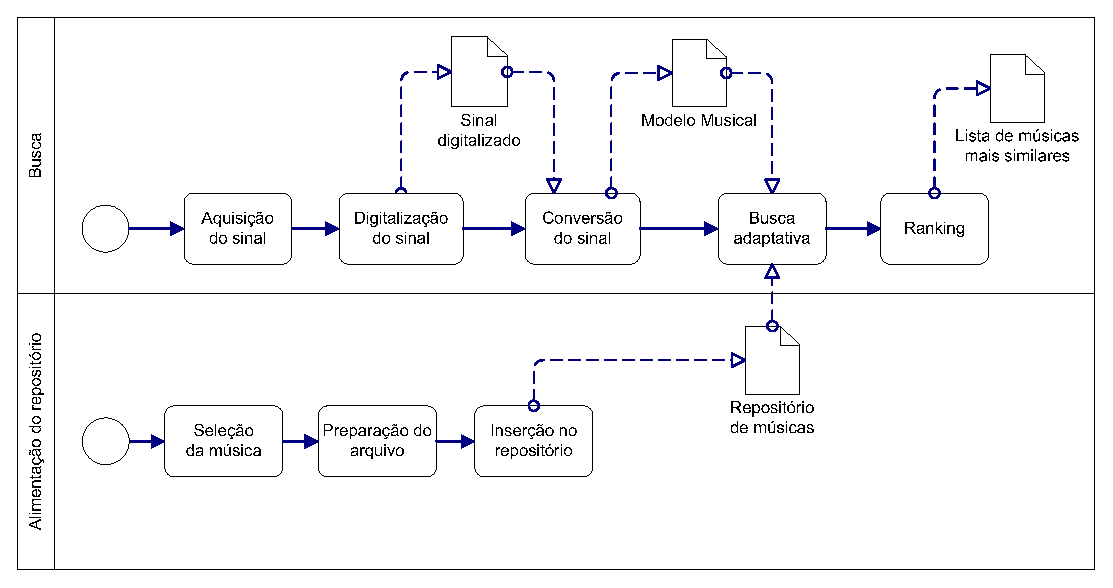
\includegraphics[width=0.9\textwidth]{figuras/fluxo.eps}}
	\caption{\label{fig:fluxo} Fluxo de informa��o do sistema}
\end{figure}

\subsubsection{Diagrama de componentes} O diagrama de componentes da Figura ~\ref{fig:componentes} mostra como as diversas partes do sistema interagem. Este diagrama � especialmente importante pois ele servir� para isolar partes do sistema, permitindo assim que os componentes evoluam separadamente, podendo-se trocar implementa��es ou m�todos utilizados sem afetar o funcionamento geral do sistema.

\begin{enumerate}

\item \emph{Aquisi��o do sinal}: � respons�vel por gravar o �udio produzido pelo usu�rio, e armazen�-lo para que o conversor em seguida possa analis�-lo. Um arquivo WAV � usado para guardar o �udio, j� que este tipo de formato apresenta perdas desprez�veis para o processo.

\item \emph{Conversor}: Receber� um sinal de �udio digitalizado, do componente anterior, e extrair� do sinal as notas cantadas pelo usu�rio, que, juntamente com suas dura��es, dar�o origem ao modelo musical que representa o �udio que o usu�rio gerou.

\item \emph{Comparador}: Recebe dois modelos musicais e os compara utilizando um aut�mato adaptativo, gerando uma medida de similaridade entre os modelos recebidos.

\item \emph{Reposit�rio}: Armazena as musicas que servem de base para a busca (em formato MIDI), e permite servi�os de gerenciamento do reposit�rio.

\item \emph{Ranking}: Ordena uma lista de m�sicas de acordo com crit�rios previamente definidos, baseando-se na similaridade e nas informa��es geradas a partir da compara��o.

\item \emph{Buscador}: A partir do modelo musical do assobio do usu�rio e das m�sicas contidas no reposit�rio, utiliza o comparador para levantar as medidas de similaridade entre o trecho recebido as m�sicas existentes no reposit�rio. Ap�s isso, utiliza-se do Ranking para ordenar a lista de m�sicas, para finalmente apresentar a resposta do sistema.

\end{enumerate}

\begin{figure}[htb]
	\center{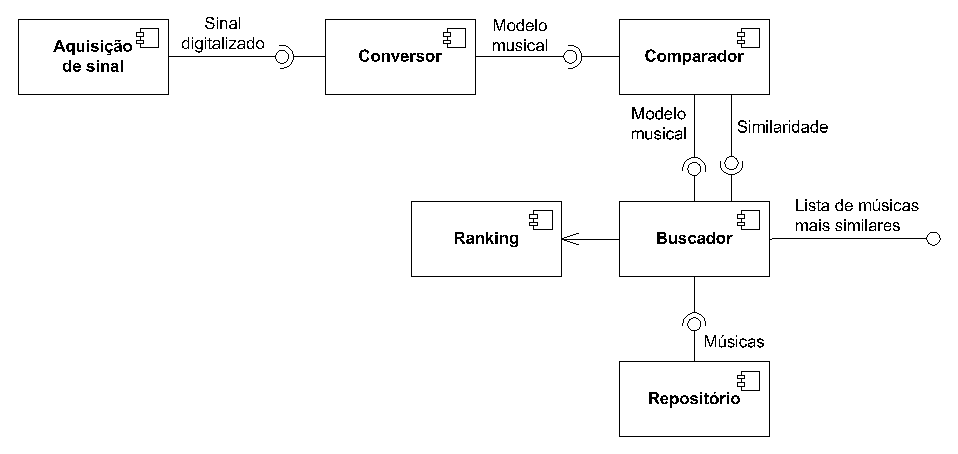
\includegraphics[width=0.9\textwidth]{figuras/componentes.eps}}
	\caption{\label{fig:componentes} Diagrama de componentes do sistema}
\end{figure}

\subsection{Escopo}

O sistema proposto � amplo e permeia diversas �reas do conhecimento, assim uma limita��o do escopo � fundamental. O foco do trabalho � a utiliza��o de t�cnicas adaptativas no reconhecimento de padr�es musicais, assim o componente de maior import�ncia � naturalmente o \emph{comparador} que � o componente que se utilizar� de tais t�cnicas. Esta � uma aplica��o inovadora, e tem o potencial de gerar bons resultados, justificando a concentra��o dos esfor�os.

Por�m, a valida��o do \emph{comparador} e a avalia��o de seu desempenho depende fundamentalmente dos dados gerados pelos outros componentes. Assim, a id�ia foi criar implementa��es simples, que fossem capazes de prover uma infra-estrutura de teste para o \emph{comparador}, por�m tal m�todo n�o foi aplic�vel a todos os componentes, como foi o caso do \emph{conversor}, exigindo um certo refino de sua implementa��o. Assim foi dada uma aten��o secund�ria ao \emph{conversor}, com o fim de poder prover dados reais de teste para o \emph{comparador}. Os outros componentes tiveram implementa��es simples, por�m suficientemente boas para prover uma prova de conceito adequada.

\section{Extra��o de notas}

A id�ia utilizada para extra��o de notas constitui da quebra o sinal de �udio em diversas janelas de tempo pequenas, extraindo-se em seguida a tranformada de Fourier destas janelas, encontrando-se assim a distribui��o de frequ�ncias para cada intervalo. A an�lise destas distribui��es permite encontrar os picos de frequ�ncia, e a partir destes picos pode-se encontrar as notas entoadas pelo usu�rio.

Assim, neste sistema o processo de extra��o de notas envolve dois componentes distintos: o componente de \emph{aquisi��o de sinal} e o \emph{conversor}, sendo constitu�do das seguintes fases:

\begin{itemize}
\item Aquisi��o do sinal
\item Extra��o do espectrograma
\item Filtro de intensidade
\item Extra��o de picos de frequ�ncia
\item Identifica��o das notas
\item Gera��o do modelo musical
\item Sintetiza��o de �udio
\end{itemize}

Estas fases s�o executadas em sequ�ncia, at� gerar a principal sa�da: o modelo musical, que prover� a entrada para o sistema de busca, enquanto o �udio sintetizado posteriormente tem o objetivo de prover um feedback do processo de extra��o de notas, permitindo avaliar a qualidade do sistema. A seguir cada uma destas fases ser�o detalhadas, mostrando as t�cnicas utilizadas em cada uma destas.

A t�cnica descrita faz parte de uma classe de m�todos baseados em an�lise de frequ�ncia, diversas abordagens similares foram desenvolvidas ao longo dos anos, em trabalhos como ~\cite{MartinPiszczalski} e ~\cite{PiszczalskiGaller}.

\subsection{Aquisi��o do sinal}
O primeiro passo para permitir o reconhecimento � a aquisi��o do sinal de �udio (assobio) gerado pelo usu�rio. Isso pode ser facilmente obtido atrav�s de um dispositivo de grava��o, como um microfone, e um software de captura de �udio. O resultado dessa etapa � armazenada em um arquivo WAV, que reproduz o assobio de forma integral.

\subsection{Extra��o do espectrograma}
A partir deste arquivo de �udio se extrai seu espectrograma, que � a transformada de Fourier para cada janela de tempo do sinal. O sinal � particionado em intervalos de tempo regulares, e para cada intervalo a dsitribui��o de frequ�ncias � calculada. O espectrograma � uma reprodu��o muito pr�xima do sinal original, por�m, transportado para o dom�nio da frequ�ncia. A fase de cada componente de frequ�ncia n�o � relevante para a an�lise, por�m sua intensidade � extremamente importante, assim, as intensidades de cada componente s�o calculadas, o resultado pode ser encarado como uma superf�cie 3D, tendo como eixo X o tempo, eixo Y a frequ�ncia e eixo Z a intensidade do sinal.

A Figura ~\ref{fig:wave} mostra o sinal de �udio original de um assobio contendo um trecho da 9.\textordfeminine \ Sinfonia de Beethoven, tamb�m conhecido como Ode � Alegria, e a Figura ~\ref{fig:espectrograma} mostra seu espectrograma. J� pelo espectrograma � poss�vel perceber os limiares das notas reproduzidas.

\begin{figure}[htb]
	\center{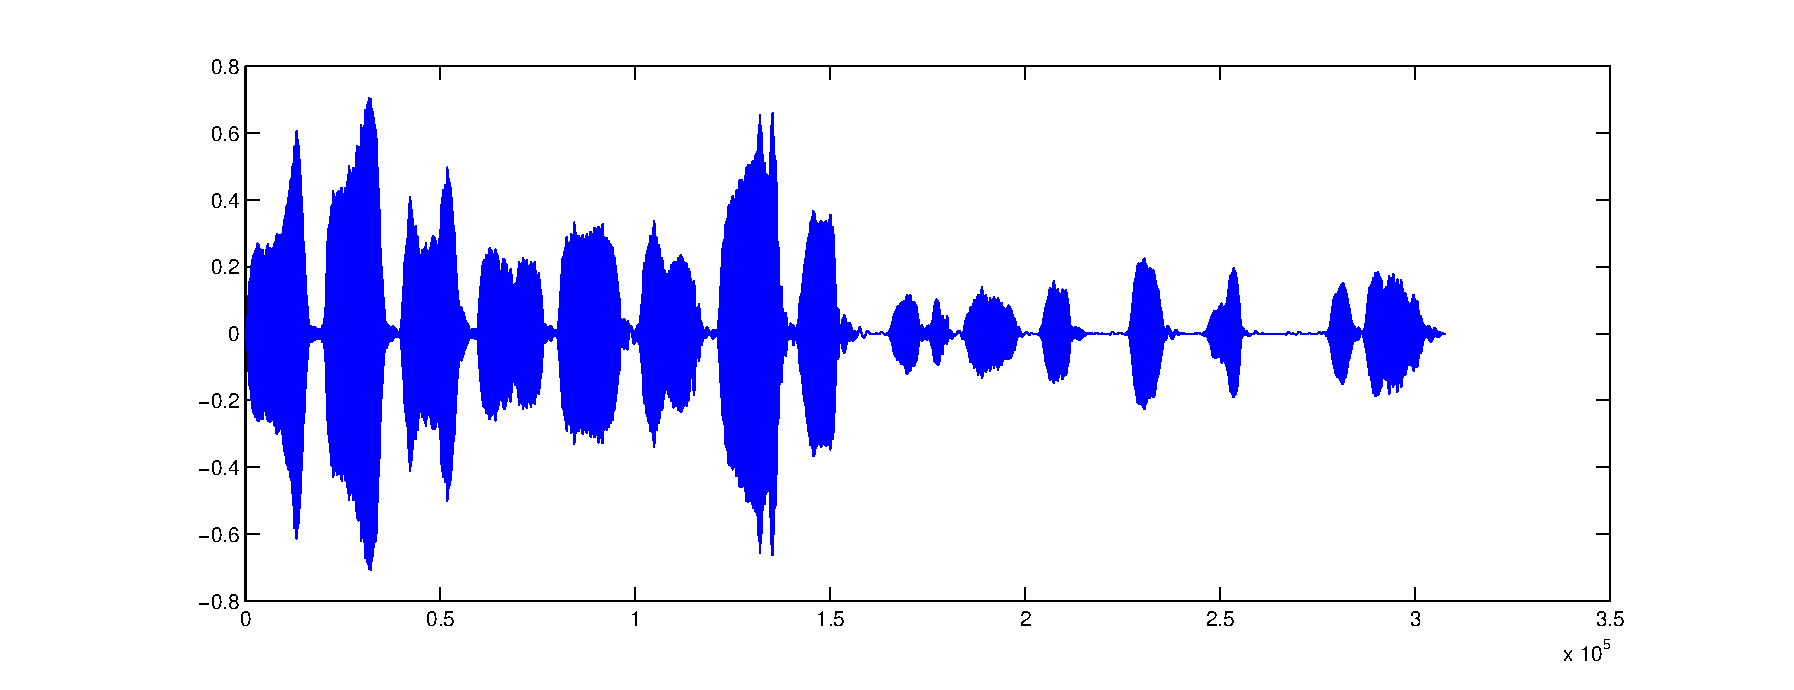
\includegraphics[width=0.7\textwidth]{figuras/ode-to-joy1-wav.eps}}
	\caption{\label{fig:wave} Sinal de �udio de um assobio}
\end{figure}

\begin{figure}[htb]
	\center{\includegraphics[width=0.7\textwidth]{figuras/ode-to-joy1-spec.eps}}
	\caption{\label{fig:espectrograma} Espectrograma do sinal correspondente a um assobio}
\end{figure}

\subsection{Filtro de intensidade}

\subsection{Extra��o de picos de frequ�ncia}

\subsection{Identifica��o das notas}

\subsection{Gera��o do modelo musical}

\subsection{Sintetiza��o de �udio}


\section{Representa��o de notas e melodias}
\label{sec:notas}
A se��o anterior descreveu o processo de extra��o de notas. Conforme foi visto, este processo analisa uma amostra de �udio de dura��o t�pica de tr�s a quinze segundos, e produz uma tabela contendo os seguintes dados sobre as notas extra�das: altura (freq��ncia fundamental de vibra��o ou \emph{pitch}) e tempos de in�cio e fim. Vale observar que nesta tabela as notas aparecem ordenadas cronol�gicamente e que n�o h� sobreposi��o temporal destas.

A representa��o tabular guarda todas as informa��es musicais da melodia extra�da e, portanto, define o formato de entrada para consultas ao mecanismo de busca musical. Por�m, internamente a este mecanismo, as melodias s�o representadas na forma de listas de eventos musicais. Neste modelo interno, um evento musical pode ser uma nota ou um sil�ncio\footnote{ou \emph{pausa}}, e guarda suas duas caracter�sticas fundamentais: altura e dura��o. A altura � mantida em \emph{Hertz} e a dura��o em segundos. Para simplificar a representa��o, adotou-se um valor zero para a altura dos sil�ncios. A ado��o desta representa��o justifica-se por uma quest�o de conveni�ncia, uma vez que os algoritmos do mecanismo de busca s�o fundamentalmente baseados em listas.

Musicalmente os sil�ncios, ou pausas, s�o considerados elementos t�o importantes quanto as pr�pias notas. Por�m analisando reprodu��es de uma mesma melodia por diferentes interpretes, nota-se uma maior simetria nos ataques\footnote{in�cios} das notas do que em seus fins. Assim, o tempo de resson�ncia das notas, e a dura��o dos sil�ncios � muito vari�vel. Ao contr�rio dos intervalos entre os ataques, que tende a se manter mais est�vel.

Conclui-se, portanto, que os intervalos entre os ataques das notas � mais relevante do que as dura��es exatas das notas e sil�ncios para defini��o da caracter�stica psicoac�stica de uma melodia. Por este motivo, para os fins deste trabalho, os sil�ncios foram eliminados das representa��es. Para manter a caracter�stica da dist�ncia temporal entre ataques de notas, a dura��o de cada sil�ncio foi incorporada � dura��o da nota imediatamente anterior.

\section{Proximidade de melodias}
Quando uma pessoa canta uma melodia ou a toca em um instrumento, somos eventualmente capazes de identificar a que m�sica aquela melodia pertence. Nosso c�rebro � capaz de reconhecer estas semelhan�as mesmo na presen�a de varia��es ou imprecis�es na melodia que ouvimos.

Um exemplo t�pico de tais varia��es � a transposi��o tonal, em que a melodia � reproduzida com uma varia��o fixa\footnote{Varia��o fixa na escala logar�tmica significa o produto por uma constante} na altura de todas as notas, para mais ou para menos. Outro exemplo � a dilata��o ou contra��o das dura��es das notas que comp�e aquela melodia.

Em muitos casos, somos capazes de identificar m�sicas mesmo na ocorr�ncia de \emph{erros} na reprodu��o, tais como uma nota errada (com altura diferente), ou mesmo a omiss�o ou adi��o de notas � melodia original. Estes erros s�o, em geral, provenientes da incapacidade ou imprecis�o do pr�prio executor.

\section{Compara��o num�rica}
Em uma situa��o hipot�tica onde n�o h� presen�a de erros, pode-se analisar a proximidade entre duas melodias com a mesma quantidade de notas, definindo um modelo matem�tico que mapeia as notas de uma melodia nas notas da outra. Sendo $p_1$ e $p_2$, respectivamente as alturas de uma nota do trecho 1 e sua correspondente no trecho 2; e $d_1$ e $d_2$ as dura��es destas; a rela��o que mapeia as dura��es � do tipo: \[ d_1 = A.d_2\]

A constante $A$ representa uma proporcionalidade entre as dura��es, portanto o modelo adotado permite dilata��es e contra��es proporcionais.

Para mapear as alturas utiliza-se a seguinte rela��o: \[ \log p_1 = \log p_2 + B \]

A constante $B$ representa a transposi��o tonal. A rela��o logar�tmica � necess�ria pelo fato de que a percep��o do ouvido humano para alturas de notas � exponencial.

A partir destas rela��es de aproxima��o, calculam-se os par�metros $A$ e $B$ que melhor aproximam a distribui��o segundo o crit�rio de proximidade do m�todo dos m�nimos quadrados, isto �, aqueles que minimizem a soma dos erros quadr�ticos:

\begin{equation} \label{E:errorDuration}
S_d = \sum_{i=1}^N (A.d_{2i} - d_{1i})^2
\end{equation}
\begin{equation} \label{E:errorPitch}
S_p = \sum_{i=1}^N (\log p_{2i} + B - \log p_{1i})^2
\end{equation}

A teoria \cite{calculoNumerico} nos mostra que o m�nimo de cada uma destas fun��es ocorre quando suas derivadas com rela��o ao par�metro atingem o valor zero:

\[ \frac{\partial S_d}{\partial A} = 0 \]
\[ 2 \sum_{i=1}^N (A.d_{2i} - d_{1i}) d_{2i} = 0 \]
\[ \sum_{i=1}^N (A.d_{2i}^2 - d_{1i}d_{2i}) = 0 \]
\begin{equation} \label{E:paramDuration}
A = \frac{\sum_{i=1}^N d_{1i}d_{2i} }{\sum_{i=1}^N d_{2i}^2 }
\end{equation}

\[ \frac{\partial S_p}{\partial B} = 0 \]
\[ 2 \sum_{i=1}^N (\log p_{2i} + B - \log p_{1i}) = 0 \]
\[ \sum_{i=1}^N (\log \frac{p_{2i}}{p_{1i}} + B) = 0 \]
\begin{equation} \label{E:paramPitch}
B = \frac { \sum_{i=1}^N \log \frac{p_{2i}}{p_{1i}} } { N }
\end{equation}

Os valores $A$ e $B$ obtidos, eventualmente podem ser utilizados para avaliar a proximidade entre as melodias. Por�m, nesta modelagem, o relevante n�o s�o os par�metros obtidos da redu��o, e sim, a soma quadr�tica dos erros ao utiliz�-los, dados pelas equa��es~\ref{E:errorDuration} e~\ref{E:errorPitch}.

Quanto menor forem os valores destas somas, mais pr�ximas s�o as melodias comparadas. A dist�ncia entre estas � ent�o definida por uma soma ponderada destes valores, com pesos ajust�veis:
\begin{equation} \label{E:distance}
d = \alpha S_d + \beta S_p
\end{equation}

\section{Busca inexata com automato adaptativo}

Com a defini��o de proximidade entre melodias apresentada acima, seria poss�vel construir um mecanismo de busca de uma melodia sobre um reposit�rio de m�sicas, utilizando uma janela deslizante do tamanho da melodia de entrada e varrendo sobre todas as melodias do reposit�rio. Por�m tal mecanismo s� seria efetivo no caso restrito em que a melodia de entrada n�o possui imperfei��es como a aus�ncia ou adi��o de notas.

Conforme j� discutido anteriormente, estas imperfei��es ocorrem com certa freq��ncia e, em condi��es habituais, n�o s�o suficientes para impedir que uma pessoa seja capaz de identificar a m�sica executada. Esta considera��o motiva a idealiza��o de um mecanismo de compara��o que seja capaz de lidar com tais imperfei��es.

No cap�tulo~\ref{chap:historico}, diversas abordagens dadas a este problema foram apresentadas. Por�m, n�o se localizou na literatura nenhum estudo que cite o uso de t�cnicas adaptativas com este fim. Prop�e-se, ent�o, um novo m�todo de reconhecimento de padr�es musicais baseado em aut�matos adaptativos.

Neste m�todo, constr�i-se um aut�mato adaptativo \cite{Neto94} automaticamente, a partir da melodia de entrada (consultada), que funciona como um reconhecedor de melodias semelhantes a esta. Este aut�mato ent�o, � utilizado para processar todo o reposit�rio de melodias e elencar as melhores semelhan�as.

Como j� foi dito anteriormente, a utiliza��o deste formalismo para a compara��o de melodias vem da necessidade de reconhecer melodias contendo imprecis�es, naturais da reprodu��o humana. Sendo assim, o aut�mato foi projetado para lidar com tr�s tipos de situa��es de erro na melodia de entrada. S�o elas:

\begin{enumerate}
\item Omiss�o de uma nota

Situa��o em que uma nota da melodia procurada foi omitida da melodia de entrada.

\item Adi��o de uma nota

Situa��o em que uma nota que n�o faz parte da melodia procurada foi inserida na melodia de entrada.

\item Troca de uma nota

Situa��o em que uma nota da melodia procurada foi substitu�da por outra qualquer na melodia de entrada.
\end{enumerate}

\section{Notas como s�mbolos}

Para ser capaz de processar melodias (tanto a da consulta como as da base de dados), o aut�mato precisa enxerg�-las na forma de cadeias de s�mbolos de um alfabeto finito. Como nesta etapa deseja-se especificamente reconhecer melodias contornando os tr�s tipos de erros enumerados anteriormente, pode-se considerar apenas a altura das notas, desprezando inicialmente as dura��es.

Por�m, os valores poss�veis de altura das notas constituem um dom�nio cont�nuo e portanto precisam ser ajustados para um dom�nio discreto, que constituir� o alfabeto do aut�mato. Para este dom�nio discreto, escolheu-se utilizar o conjunto de alturas das notas de um piano. Este conjunto, conhecido musicalmente como \emph{temperamento igual de 12 tons}, � o sistema de afina��o predominantemente utilizado na m�sica ocidental moderna \cite{Burns99}.

O MIDI\footnote{Musical Instrument Digital Interface} \cite{midi} � um padr�o de facto que define um protocolo para comunica��o entre instrumentos musicais eletr�nicos e outros equipamentos de �udio. Entre os diversos outros detalhes do protocolo, o MIDI define um c�digo para representa��o das notas do sistema de afina��o ocidental (notas do piano). Este c�digo � um n�mero inteiro entre 0 e 127, que � capaz de representar muito al�m da capacidade aud�vel da maioria dos seres humanos. A nota 0, por exemplo, � uma nota D� cinco oitavas abaixo do D� central e corresponde a uma freq��ncia de 8,176 Hz. Por conveni�ncia, adotaremos este c�digo de notas MIDI como alfabeto do aut�mato.

A primeira etapa do ajuste de dom�nio � basicamente uma convers�o de unidades. A convers�o da altura em Hertz para o c�digo MIDI � dada pela seguinte rela��o:
$$ p = 69 + 12\times\log_2 { \left(\frac {f}{440\,\mbox{Hz}} \right) }. $$

Ap�s esta convers�o � necess�rio realizar uma quantiza��o a fim de obter valores inteiros, discretizando o dom�nio. Note, por�m, que este processo n�o � t�o simples quanto um arredondamento. Pois o que define a caracter�stica perceptiva de uma melodia � a rela��o entre as alturas das notas e n�o seus valores absolutos, haja visto que a transposi��o tonal n�o altera esta caracter�stica. Sendo assim, um simples arredondamento poderia ocasionar erros de quantiza��o consider�veis.

Outro aspecto a se considerar � que o executor da melodia, pode perder a refer�ncia absoluta de afina��o durante sua reprodu��o. Ou seja, para uma melodia suficientemente grande, a refer�ncia de afina��o para uma determinada nota vem das $k$ notas anteriores e n�o da melodia inteira.

Considerando este aspecto relativo da reprodu��o humana, uma pesquisa da Universidade de Waikato (Nova Zel�ndia) apresentou um simples e interessante m�todo de quantizar estes valores a partir da refer�ncia de afina��o da nota anterior.

Este m�todo foi reproduzido e testado utilizando valores extra�dos de grava��es de melodias assobiadas. Por�m, os resultados mostraram que, em alguns casos, ocorre uma diverg�ncia elevada, maior que eventuais varia��es da refer�ncia absoluta do executor. O gr�fico da figura~\ref{fig:quant-rel} ilustra um destes casos.

\begin{figure}[htb]
	\center{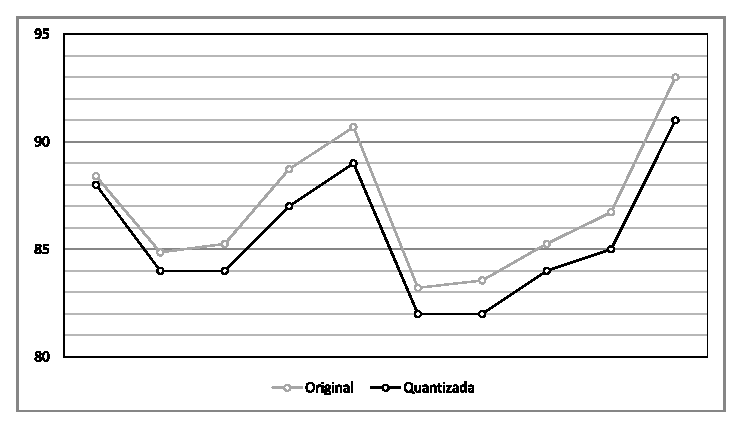
\includegraphics{figuras/quant-rel.eps}}
	\caption{\label{fig:quant-rel} Alturas quantizadas pelo m�todo relativo}
\end{figure}

Tendo em vista as limita��o deste m�todo de quantiza��o relativo, foi desenvolvido um m�todo de quantiza��o absoluto que ser� descrito em detalhes na se��o seguinte.

\subsection{Quantiza��o absoluta das alturas das notas}

O m�todo proposto parte do princ�pio que a melodia original pode ser transposta de tonalidade livremente, ou seja, pode-se somar uma constante em todas as notas sem que o resultado da quantiza��o perca significado. A partir disto encontra-se analiticamente a constante que minimiza uma m�trica de erro de quantiza��o e, por fim, faz-se o arredondamento das notas somadas a esta constante.

A soma do erro quadr�tico de quantiza��o por arredondamento � dada por:
\[ E(0) = \sum_{i=1}^N (p_i - \lfloor p_i + \frac{1}{2} \rfloor)^2\]

Com a adi��o de uma constante $c$ em todos os valores, torna-se:
\[ E(c) = \sum_{i=1}^N (p_i + c - \lfloor p_i + c + \frac{1}{2} \rfloor)^2\]

Este valor varia com a constante $c$. Em suma, queremos encontrar o valor de $0 < c \leq 1$ que minimiza $E$, para ent�o obter os valores quantizados $v_i$ da seguinte maneira:
\[ v_i = \lfloor p_i + c + \frac{1}{2} \rfloor.\]

Note que a fun��o $E$ n�o � cont�nua. Por este motivo, seu m�nimo pode estar ou nos pontos de descontinuidade ou nos pontos em que:
\begin{equation} \label{E:dE}
\frac{\partial E}{\partial c} = 0.
\end{equation}

Os pontos de descontinuidade ocorrem quando $c = \frac{1}{2} + \lfloor p_i + \frac{1}{2} \rfloor - p_i + k$, $k \in \mathbb{Z}$, para qualquer $p_i$. Estes pontos s�o candidatos a m�nimo de $E$. Entre dois destes pontos consecutivos $c_1$ e $c_2$, $E$ � cont�nua e ent�o podemos desenvolver a equa��o ~\ref{E:dE}:
\begin{equation} \label{E:dE2}
\sum_{i=1}^N (p_i + c - \lfloor p_i + c + \frac{1}{2} \rfloor) = 0
\end{equation}

Por termos restringido o intervalo para uma regi�o cont�nua, o termo $\lfloor p_i + c + \frac{1}{2} \rfloor$ agora passa a ser constante. Para calcul�-lo basta utilizar para $c$ um valor qualquer do intervalo, como por exemplo a m�dia dos extremos:
$$ \bar{c} = \frac{c_1+c_2}{2}$$

Com isso a equa��o ~\ref{E:dE2} fica:
\begin{equation} \label{E:dE3}
c = \frac { \sum_{i=1}^N (\lfloor p_i + \bar{c} + \frac{1}{2} \rfloor - p_i) } { N }
\end{equation}

Se o valor obtido para $c$ estiver no intervalo $\left]c_1,c_2\right[$ este ser� solu��o da equa��o ~\ref{E:dE} e, portanto, um novo canditado a m�nimo de $E$.
Aplica-se este procedimento para todos os trechos entre pontos de descontinuidade do intervalo $\left]0,1\right]$ e obtem-se desta forma todos os candidatos a m�nimo de $E$. Basta verificar os valores de $E$ para cada candidato e escolher aquele que a minimiza.

O gr�fico da figura~\ref{fig:quant-cmp} mostra uma compara��o dos resultados dos dois m�todos de quantiza��o utlizando a mesma melodia da figura~\ref{fig:quant-rel}.

\begin{figure}[htb]
	\center{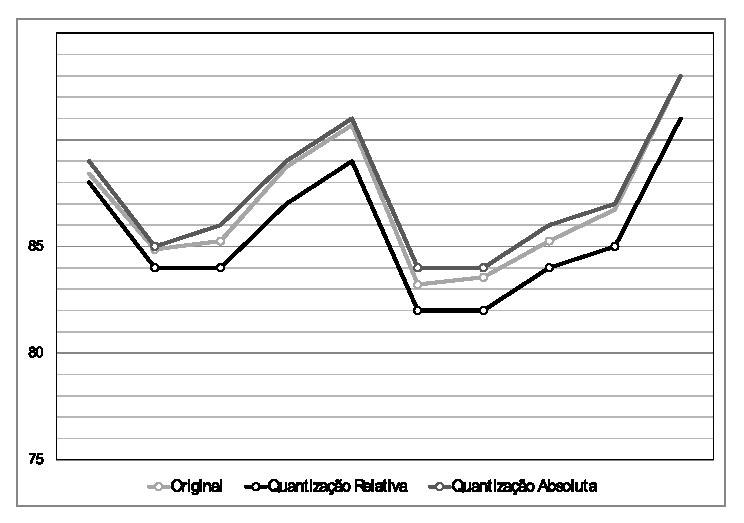
\includegraphics{figuras/quant-cmp.eps}}
	\caption{\label{fig:quant-cmp} Compara��o dos dois m�todos de quantiza��o de alturas}
\end{figure}

\subsection{Constru��o do aut�mato adaptativo}
	
A configura��o inicial do aut�mato adaptativo � obtida atrav�s da cadeia de entrada do processo de busca, isto �, a cadeia a ser localizada no reposit�rio. Seja a cadeia de entrada $v_i$, $i=0,\ldots,N-1$. O aut�mato � constru�do inicialmente com $N+1$ estados, numerados de $0$ a $N$, onde apenas o estado $N$ � final. Adiciona-se transi��es do estado $i$ para o estado $i+1$ com o s�mbolo $v_i$, para $i=0,\ldots,N-1$.

Para ilustrar o funcionamento do aut�mato, considere a seguinte seq��ncia de notas: 69, 71, 73, 74, 76, 77, 76. A figura~\ref{fig:adapt1} mostra a configura��o inicial do aut�mato adaptativo gerado para esta seq��ncia.

\begin{figure}[htb]
	\center{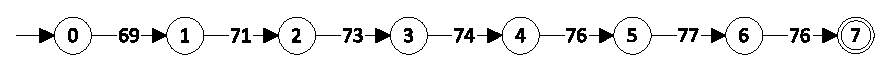
\includegraphics{figuras/adapt1.eps}}
	\caption{\label{fig:adapt1} Configura��o inicial do aut�mato adaptativo}
\end{figure}

A execu��o do aut�mato sobre uma cadeia qualquer inicia-se com o c�lculo de uma constante de transposi��o. Esta constante nada mais � do que a diferen�a entre a primeira nota da cadeia de entrada e a da cadeia que originou o aut�mato. Este valor � descontado dos s�mbolos de entrada a cada leitura, e serve fundamentalmente para desfazer uma poss�vel transposi��o tonal.

O caminho definido pelos estados de $0$ a $N$, deste ponto adiante chamado de caminho de refer�ncia, ocorre quando a cadeia de entrada equivale exatamente � cadeia procurada, a menos da constante de transposi��o.

Estando no caminho de refer�ncia, ao receber um s�mbolo para o qual n�o existe transi��o, ocorre uma a��o adaptativa em que uma estrutura de novos estados e transi��es � incorporanda ao aut�mato a partir do estado corrente.

Suponha que o aut�mato da figura~\ref{fig:adapt1} recebeu na entrada as notas 69 e 71, atingindo o estado 2. Em seguida, o aut�mato recebeu o s�mbolo 74 e disparou a a��o adaptativa. A figura~\ref{fig:adapt2} mostra a configura��o deste aut�mato ap�s esta a��o.

\begin{figure}[htb]
	\center{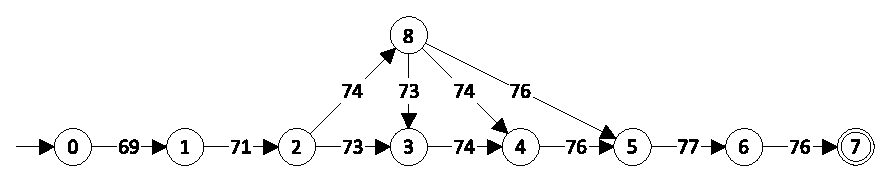
\includegraphics{figuras/adapt2.eps}}
	\caption{\label{fig:adapt2} Configura��o do aut�mato ap�s a��o adaptativa 1}
\end{figure}

O aut�mato atinge o novo estado 8 e, a partir das novas transi��es incorporadas, torna-se capaz de lidar com as tr�s situa��es de erro.
\begin{enumerate}
\item Omiss�o de uma nota

Se a nota 74 recebida fora omitida da cadeia que gerou o aut�mato, o reconhecimento volta para o caminho de refer�ncia a partir do estado 3 ao receber a nota 73, que esperava anteriormente.

\item Adi��o de uma nota

Se a nota 73, que era esperada, fora inserida erroneamente na cadeia que gerou o aut�mato, o reconhecimento volta para o caminho de refer�ncia a partir do estado 5 ao receber a pr�xima nota da seq��ncia: 76.

\item \label{i:troca} Troca de uma nota

Se a nota 74 fora trocada por engano pela 73 na cadeia que gerou o aut�mato, o reconhecimento volta para o caminho de refer�ncia a partir do estado 4 ao receber a nota seguinte: 74.
\end{enumerate}

Note que o caso de adi��o de uma nota s� p�de ser contornado por que a nota recebida coincidiu com a segunda nota esperada do aut�mato. Quando isto n�o ocorrer, a transi��o que contorna este caso n�o � gerada. Um exemplo desta situa��o pode ser observado na figura~\ref{fig:adapt3}.

\begin{figure}[htb]
	\center{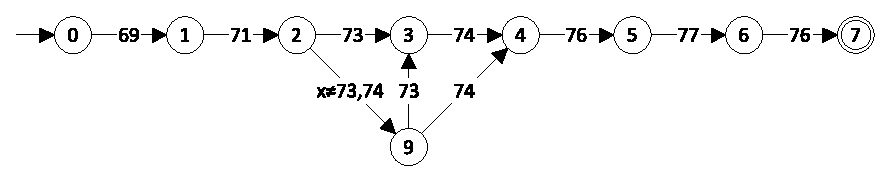
\includegraphics{figuras/adapt3.eps}}
	\caption{\label{fig:adapt3} Configura��o do aut�mato ap�s a��o adaptativa 2}
\end{figure}

� importante observar que este aut�mato � capaz de reconhecer melodias contendo m�ltiplos erros, desde que devidamente espa�ados. A ocorr�ncia de dois erros consecutivos implica na n�o aceita��o da cadeia, pois n�o h� a��es adaptativas nos estados fora do caminho de refer�ncia. Tal possibilidade implicaria em um tratamento muito mais complexo das possibilidades de combina��o de erros e transi��es de recupera��o.

Uma limita��o importante deste tipo aut�mato � percebida em situa��es em que as transi��es de recupera��o de erro s�o conflitantes. No exemplo apresentado, as transi��es de recupera��o de erro s�o indepententes, por serem disparadas com s�mbolos diferentes. Por�m, em alguns casos, quando as melodias possuem notas repetidas, transi��es de recupera��o diferentes podem ser disparadas com um mesmo s�mbolo. Neste casos, para evitar o n�o-determinismo do aut�mato, elimina-se a transi��o de menor prioridade. Os casos de erro em ordem decrescente de prioridade s�o: adi��o, troca e omiss�o.

Durante o reconhecimento de uma cadeia, o aut�mato registra um c�digo de resultado para cada nota lida, em uma lista. Quando a nota recebida era esperada, o algoritmo registra \texttt{OK}. Quando a nota n�o era esperada o algoritmo registra o c�digo da situa��o de erro ocorrida: \texttt{EXCHANGE}, \texttt{ADDITION} ou \texttt{OMISSION}. Note que neste caso o resultado depende da transi��o de recupera��o que for utilizada e s� pode ser determinado ao tratar a nota seguinte.

Quando o aut�mato atinge o estado final, a cadeia � considerada aceita e a lista de c�digo de resultado representa os detalhes do reconhecimento. Caso contr�rio, a cadeia � rejeitada, por�m, para se saber at� que ponto a cadeia foi reconhecida retorna-se a lista de c�digo de resultado parcial. Esta lista cont�m os resultado at� o momento em que a cadeia foi rejeitada.

Abaixo segue uma simula��o de execu��o do aut�mato da figura~\ref{fig:adapt1}, para cadeias de entrada contendo cada uma das tr�s situa��es de erro descritas a pouco. Primeiramente mostra-se a cadeia utilizada para constru��o do aut�mato. Esta cadeia representa a consulta ao sistema de busca. Em seguida, entra-se com cadeias para serem processadas pelo aut�mato, representando trechos de melodias da base de dados. Para cada entrada o aut�mato retorna a lista de c�digos de resultado.

\begin{listagem}
\begin{verbatim}
Cadeia para produzir o aut�mato:
69 71 73 74 76 77 76 0

Exemplo de troca:
69 71 74 74 76 77 76 0
[OK, OK, EXCHANGE, OK, OK, OK, OK]

Exemplo de adi��o:
69 71 74 76 77 76 0
[OK, OK, ADDITION, OK, OK, OK]

Exemplo de omiss�o:
69 71 72 73 74 76 77 76 0
[OK, OK, OMISSION, OK, OK, OK, OK, OK]
\end{verbatim}
\caption{Resumo da simula��o de execu��o do aut�mato}
\end{listagem}


\begin{listagem}
\begin{verbatim}
Entre com uma cadeia terminada por 0 para gerar o aut�mato:
69 71 73 74 76 77 76 0
Digite:
	1, para digitar uma cadeia de entrada.
	2, para gerar uma cadeia de entrada.
	0, para sair.
1
Entre com a cadeia de entrada terminando com 0:
69 71 74 74 76 77 76 0
true
[OK, OK, EXCHANGE, OK, OK, OK, OK]
Digite:
	1, para digitar uma cadeia de entrada.
	2, para gerar uma cadeia de entrada.
	0, para sair.
1
Entre com a cadeia de entrada terminando com 0:
69 71 74 76 77 76 0
true
[OK, OK, ADDITION, OK, OK, OK]
Digite:
	1, para digitar uma cadeia de entrada.
	2, para gerar uma cadeia de entrada.
	0, para sair.
1
Entre com a cadeia de entrada terminando com 0:
69 71 72 73 74 76 77 76 0
true
[OK, OK, OMISSION, OK, OK, OK, OK, OK]
Digite:
	1, para digitar uma cadeia de entrada.
	2, para gerar uma cadeia de entrada.
	0, para sair.
\end{verbatim}
\caption{Sa�da completa da simula��o de execu��o do aut�mato}
\end{listagem}

Uma cadeia ser aceita pelo aut�mato significa na pr�tica que contornando eventuais situa��es de erro devidamente isoladas as cadeias s�o semelhantes. A partir deste momento a lista de c�digos de resultados � analisada com o objetivo de mensurar a dist�ncia entre as cadeias comparadas.

Para esta an�lise, dois aspectos s�o considerados. O primeiro deles � direto e correponde � quantidade de erros observados. Quanto menor o n�mero de erros mais pr�ximas s�o as cadeias. O segundo aspecto envolve um procedimento mais elaborado. Note que a partir da cadeia que originou o aut�mato e da lista de c�digos de resultados, � poss�vel construir uma cadeia artificial, corrigindo os erros registrados. Assim se, por exemplo, uma nota for omitida, pode-se readicion�-la � cadeia. O objetivo desta reconstru��o � possibilitar a aplica��o dos m�todos num�ricos de compara��o nota a nota apresentados anteriormente. Principalmente com rela��o �s dura��es das notas, aspecto que fora desconsiderado nesta nova abordagem at� ent�o.

Algumas considera��es s�o importantes no que tange � reconstru��o da cadeia com base nas informa��es de erros. Para notas trocadas deve-se manter a dura��o original. Para notas omitidas, estas dever�o ser readicionadas com dura��o zero para que n�o haja interfer�ncia no contorno temporal geral da cadeia. A nota � adicionada somente para alinhar o emparelhamento necess�rio para a compara��o nota a nota. E, por fim, para o o caso de notas adicionadas, estas s�o retiradas e sua dura��o � incorporada � nota imediatamente anterior.

Com base nestas considera��es constr�i-se a cadeia corrigida e, executando o procedimento de compara��o de dura��es, consegue-se obter uma nova m�trica de dist�ncia entre as melodias, desta vez utilizando m�todos num�ricos e considerando as dura��es das notas.

\subsection{Crit�rio para avaliar a semelhan�a entre melodias}

Com o modelo de compara��o que foi definido, tem-se algumas m�tricas para avalia��o da semelhan�a entre melodias. A primeiras delas � se o aut�mato chegou ou n�o ao estado final. Outra m�trica � representada pela lista de c�digos de resultado e, por fim, a dist�ncia num�rica das dura��es.

Existe uma rela��o de import�ncia que cada um destes fatores t�m sobre a semelhan�a global percebida. Por�m, a falta de testes massivos impede uma percep��o apurada destas import�ncias e por conseq��ncia impossibilita a atribui��o de pesos para cada fator.

Por�m, faz-se necess�rio definir um crit�rio simples e direto com o objetivo de classificar as correspondencias encotradas. Adotou-se para este fim a contagem dos erros a partir da lista de c�digos de resultado. Para as listas parciais (quando a cadeia n�o � aceita), somou-se � contagem de erros o n�mero de notas que sobraram no momento em que o reconhecimento parou.

\subsection{Busca}

Sumarizando o procedimento de busca, temos inicialmente a constru��o do aut�mato adaptativo a partir da melodia de entrada quantizada. Em seguida aplica-se o aut�mato sobre todas as melodias do reposit�rio. Este � aplicado inicialmente � cadeia que corresponde a uma melodia completa. Em seguida, a primeira nota desta cadeia � eliminada e o aut�mato � aplicado novamente. E assim sucessivamente at� que a cadeia torne-se vazia, ent�o parte-se para a pr�xima melodia do reposit�rio.

Ao longo deste processo, o mecanismo de busca mant�m um conjunto com as N melhores correspond�ncias que encontrou, com base no crit�rio definido a pouco. Desta forma, ao final da varredura de todo o reposit�rio, tem-se os resultados da busca.


\chapter{Resultados}
\chapter{An�lise}
\chapter{Cr�tica}
\chapter{Melhorias e Trabalhos futuros}

Desde o in�cio a proposta do trabalho era desenvolver uma t�cnica de compara��o de conte�dos de �udio utilizando uma tecnologia adaptativa, associado a um prot�tipo funcional que fosse capaz de exercitar e avaliar a t�cnica de compara��o desenvolvida, assim, diversos pontos do trabalho foram abordados apenas superficialmente, e s�o pass�veis de grandes melhorias. A seguir ser�o apresentados alguns dos pontos de extens�o mais importantes.

\paragraph*{Automatiza��o da identifica��o de notas.} O processo executado no trabalho foi manual, e � pass�vel de automatiza��o, para tanto, a an�lise das varia��es de intensidade e varia��es de frequ�ncia ao longo da linha de tempo podem ser extremamente �teis. Pode-se utilizar como base trabalhos j� desenvolvidos, a fim de melhorar esta fase do prot�tipo.

\paragraph*{Maior granularidade de erros.} Foram considerados apena tr�s tipos de erros para este trabalho (\emph{OMISS�O}, \emph{ADI��O} e \emph{TROCA} de uma nota), ao longo do desenvolvimento percebeu-se que estas classes de erro apenas n�o s�o capazes de contabilizar com precis�o o desvio que o usu�rio tenha cometido, assim prop�em-se a cria��o de uma nova classe de erro, denominada \emph{VARIA��O MENOR}, que seria similar � uma \emph{TROCA}, por�m representaria uma troca pequena, dentro de uma toler�ncia pr�-determinada. Esta nova classe tem o objetivo de descrever um erro muito comum, onde o usu�rio n�o troca uma nota por completo, mas sim desvia um pouco da nota original, por exemplo, ao subir um tom apenas.

\paragraph*{M�ltiplos erros.} O aut�mato desenvolvido � capaz de lidar com erros simples apenas (dentro da defini��o proposta), por�m � extremamente comum, em especial para o caso de \emph{TROCA}, que o usu�rio cometa mais de erro seguido. O projeto atual do aut�mato n�o � capaz de lidar e aceitar m�ltiplos erros, gerando \emph{scores} mais baixos do que o esperado para trocas seguidas.

\paragraph*{Defini��o dos pesos de cada classe de erro.} Para a gera��o do grau de similaridade, diversos fatores devem ser levados em considera��o, como:

\begin{itemize}
\item N�mero de erros
\item Tipos de erros cometidos
\item Aceita��o ou n�o da cadeia (atingir o fim do aut�mato)
\end{itemize}

Tais fatores influenciam diferentemente na similaridade entre dois conte�dos, por exemplo, a omiss�o de uma nota � intuitivamente um erro mais grave do que uma pequena troca de uma nota. Por�m, essas diferen�as de erros n�o s�o contabilizadas, sendo tratadas da mesma forma. Testes com reposit�rios maiores e associados a um \emph{feedaback} humano poderia prover dados que ajudassem a calibra��o dos pesos de cada fator no \emph{score} final.
\chapter{Contribui��es}

% $Id: bibliografia.tex,v 1.1 2003/04/10 23:12:59 gweber Exp $
%%%%%%%%%%%%%%%%%%%%%%%%%%%%%%%%%%%%%
%% Bibliografia
%% Copyright 2003 Dehon Charles Regis Nogueira.
%% Este documento � distribu�do nos termos da licen�a
%% descrita no arquivo LICENCA que o acompanha.
%%%%%%%%%%%%%%%%%%%%%%%%%%%%%%%%%%%%%

\nocite{*}

\bibliographystyle{abnt-alf}
\bibliography{biblio}



\end{document}

